% !TEX root = ../../../main.tex
% 来源：高中物理甲种本·第三册（电磁·光学·近代物理）
% 章节：交流电 / 交流电的变化规律
% 原始文件：3.tex，行 189-205
% 类型：tikz
% ---
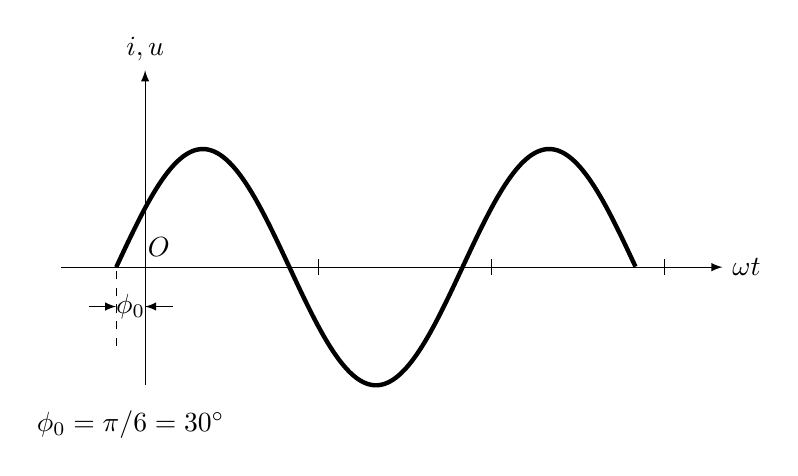
\begin{tikzpicture}[>=latex, xscale=.7]

\draw[->] (-1,0)--(11,0)node [right]{$\omega t$};
\draw[->] (3.1416/6, -1.5)--(3.1416/6, 2.5)node [above]{$i,u$};
\foreach \x in {3.1416*7/6, 3.1416*13/6, 3.1416*19/6}
{
   \draw (\x, -.1)--(\x, .1);
}
\draw [ultra thick] plot[domain=0:3*3.1416, samples=1000, variable=\x] (\x, {1.5*sin(\x r)}) ;
\draw[dashed](0,-1)--(0,0);

\node at (3.1416/12, -.5){$\phi_0$};
\node at (3.1416/12, -2){$\phi_0=\pi/6=30^{\circ}$};
\draw[->] (-.5,-.5)--(0,-.5);
\draw[->] (3.1416/6+.5,-.5)--(3.1416/6,-.5);
\node at  (3.1416/6+.25,.25) {$O$};
\end{tikzpicture}
